%% Example of a LaTeX source file for a COLING-2012 submission
%% last updated: July 10, 2012
%% Optional instructions for authors within the tex file are provided as comments and start with 'for authors:...'
\documentclass[10pt,a5paper,twoside]{article}
\usepackage{coling2012}
\usepackage{comment}
\usepackage{amsmath}
%\title{Translating to Shakespeare: A Case Study in Paraphrasing Writing Styles}
%\title{You can be Shakespeare! \\ A Case Study in Paraphrase Targeting Writing Styles}
%\title{A rose would smell just as good even if it had a different name (``A rose by any other name would smell as sweet'') \\ A Case Study in Paraphrase Targeting Writing Styles}
%\title{“Be super careful on March 15” (“Beware the ides of March”) \\ A Case Study in Paraphrase Targeting Writing Styles}
\title{``A rose by any other name would smell as sweet'': \\ A Case Study in Paraphrase Targeting Writing Styles}
%for authors: in case of more than four author names ref. to commented line below 
%\author{$Annie~SMITH^{1, 2}~~~LI~Xiao Dong^{1, 3}$\\$~~~Third~Author^{1, 2}~~~Fourth~Author^{1, 3}~~~ Fifth~Author^{2, 3}$\\
\author{$Author1^{1, 2}~~~Author2^{1, 3}$\\
{\small  	(1) INSTITUTE\_1, address 1\\ 
 		(2) INSTITUTE\_2, address 2\\
		(3) INSTITUTE\_3, address 3\\
  \texttt{author1@institute1, author@institute2} \\ 
}}

\begin{document}
\maketitle
%% The first mandatory ABSTRACT (\abstractEn) section below is for the English language
\abstractEn{  %ABSTRACT}{
We present initial investigation into the task of paraphrasing language while targeting a particular writing style.
The plays of William Shakespeare and their modern translations are used as a testbed for evaluating
paraphrase systems targeting a specific style of writing.
%We demonstrate that existing evaluation metrics developed in the Machine Translation and Paraphrase communities are
%insufficient when the goal is to generate paraphrases targeting a specific style, and
%propose a series of new metrics to measure how closely the generated paraphrases match the target
%style.  
We show that even with a relatively small amount of parallel training data available, it is
possible to learn paraphrase models which capture stylistic phenomenon, and these models outperform
baselines based on dictionaries and out-of-domain parallel text.
In addition we present an initial investigation into automatic evaluation metrics for paraphrasing writing style.
To the best of our knowledge this is the first work to investigate the task of
paraphrasing text with the goal of targeting a specific style of writing.
}

\keywordsEn{Paraphrase, Writing Style}

\newpage
\section{Introduction}
%The plays of William Shakespeare and their \emph{modern} translations are treated
%as parallel text which is used to learn paraphrase models targeting the style of Early Modern English employed by Shakespeare.

The same meaning can be expressed or \emph{paraphrased} in many different ways; automatically detecting or generating different expressions with the same meaning is 
fundamental to many natural language understanding tasks\cite{Giampiccolo07}, so much previous work has investigated methods for automatic paraphrasing\cite{Barzilay03,dolan04,Shinyama03,Das09,bannard05}.  

Paraphrases can differ along many dimensions, including utterance length, diction level, and speech register. 
There is a significant literature in sentence compression aimed at modeling the first of these, length: 
producing meaning-preserving alternations that reduce the length of the input string {\bf TODO:} [citations].
However, we know of no previous work aimed at modeling meaning-preserving transformations that systematically transform the register or style of an input string. 
Can we learn to reliably map from one form of language to another, transforming formal prose into a more colloquial form, or a casual email into a more formal equivalent?

%Although two utterances may be semantically equivalent, they can still be stylistically quite different.  For example, the same information
%is likely to be conveyed using very different lexical and grammatical patterns in advertising materials v.s. technical manuals, or in Shakespearean plays v.s. Hollywood movies.

Systems capable of paraphrasing text targeting a specific writing style could be useful for a variety of applications.  For example, they could:
\begin{enumerate}
  \item Help authors of technical documents to adhere to appropriate stylistic guidelines.  
  \item Enable average people to better consume information by translating legalese or medical jargon into nontechnical English.  
  \item Benefit educational applications, allowing students to:
    \begin{enumerate}
    \item Access \emph{modern English} versions of works by authors they are studying.
    \item Experiment with writing in the style of an author they are studying.
    \end{enumerate}
\end{enumerate}

In this paper, we investigate the task of automatic paraphrasing techniques that target a particular writing style, focusing specifically on the style of Early Modern English employed by William Shakespeare.
We explored several different methods, all of which rely on techniques from phrase-based MT, but which were trained on different types of parallel monolingual data.  The first engine was trained on the text of Shakespeare’s plays, along with parallel modern English “translations” that were written to help students better understand Shakespeare's work.  
%A parallel corpus is extracted from these modern translations,
%which is then used to train phrase-based translation models which are capable of automatically paraphrasing ordinary sentences into Shakespearean English.  
We also developed several
baseline systems which do not make use of this parallel text and instead rely on manually compiled dictionaries of expressions commonly found in Shakespearean English, or existing
corpora of out-of-domain parallel monolingual text.

We evaluate these models both through human judgments and standard evaluation metrics from the Machine Translation (MT) and Paraphrase literature, however no previous work has investigated the ability of automatic
evaluation metrics to capture the notion of writing style.  
We show that previously proposed metrics do not provide the complete picture of a system's performance when the task is to generate paraphrases
targeting a specific style of writing.  We therefore propose two new metrics for evaluating paraphrases targeting a specific style, and 
show that these metrics correlate well with human judgments.

\begin{comment}
Systems which are capable of automatically paraphrasing literary writing styles could be directly beneficial for educational applications.  For example, our systems which generate paraphrases targeting
Shakespearean English could help students to experiment with writing literature in this style.
In addition, out of the 37 surviving plays written by William Shakespeare, modern translations are currently only available for 17.  
We therefore present a preliminary investigation into the task of automatically translating Shakespeare's plays into modern English, using our newly developed
automatic evaluation metrics.  By automatically paraphrasing the remaining 20 plays into modern English, 
we believe it should be possible to help make these plays more accessible to students of Shakespeare.
\end{comment}

\section{Shakespearean Paraphrasing}
We use Shakespeare's plays as a testbed for the task of paraphrasing while targeting a specific writing style.  Because these plays are some of 
the most highly-regarded examples of English literature and 
are written in a style that is now 400 years out of date, many linguistic resources are available to help modern readers pick their way through 
these Elizabethan texts. Among these are “translations” of the plays into colloquial English, as well as dictionaries that provide modern equivalents for archaic words and phrases.

We compare 3 different stylistic paraphrase systems targeting Shakespearean English which rely on different types of linguistic resources. 
One leverages parallel “translations”, another exploits dictionary resources, and a third relies on modern, out-of-domain monolingual parallel data and an in-domain corpus.

\subsection{Modern Translations}
\label{modern_translations}
Access to parallel text in the target style allows us to train statistical models that generate paraphrases, and also perform automatic evaluation of semantic adequacy using BLEU, which requires availability of reference translations.  For this purpose we scraped modern translations of 17 Shakespeare plays from \url{http://nfs.sparknotes.com}, and 
additional translations of 8 of these plays from \url{http://enotes.com}.

After tokenizing and lowercasing, the plays were sentence aligned \cite{Moore02}, producing 21,079 alignments from the 31,718 sentence pairs in the Sparknotes data, and 10,365 sentence pairs from the 13,640 original 
pairs in the Enotes data.  The modern translations from the two sources are qualitatively quite
different.  The Sparknotes paraphrases tend to differ significantly from the original text, whereas the Enotes translations are much more conservative, making fewer changes.
To illustrate these differences empirically and provide an initial paraphrase baseline, we computed BLEU scores of the modern translations against Shakespeare's 
original text; the Sparknotes paraphrases yield a BLEU score of 24.67, whereas the Enotes paraphrases produce a much higher BLEU of 52.30 reflecting their strong similarity to the original texts.
These results are summarized in Table \ref{corpus_stats}.

\begin{table}
  \begin{center}
    \begin{tabular}{|l|r|r|r|}
      \hline
      corpus & initial size & aligned size & No-Change BLEU\\
      \hline
      \hline
      \url{http://nfs.sparknotes.com} & 31,718 & 21,079 & 24.67 \\
      \hline
      \url{http://enotes.com} & 13,640 & 10,365 & 52.30 \\
      \hline
    \end{tabular}
  \end{center}
  \caption{Parallel corpora generated form modern translations of Shakespeare's plays}
  \label{corpus_stats}
\end{table}

To generate paraphrases, we applied a typical phrase-based statistical MT pipeline, performing
word alignment on the data described in table \ref{corpus_stats} using GIZA++ \cite{Och03}, then extracting phrase pairs and performing decoding using Moses \cite{Koehn07}.

For evaluation purposes, the parallel text of one play, Romeo and Juliet, was held out of the training corpus for this system and the baseline systems described in the following section.

\subsection{Baselines}
Phrase-based translation has been demonstrated as an effective approach to paraphrasing \cite{quirk04,chen11}.  However, this approach does require the existence of
parallel corpora of aligned phrases and sentences, resources which may not be available for many writing styles that we might wish to target.  For this reason we were motivated to investigate alternative approaches in order to help
quantify how critical this type of parallel data is for the task of stylistic paraphrasing.

\subsubsection{Dictionary Based Paraphrase}
\label{dictionary_baseline}
Several dictionaries of stylistically representative words of Shakespearean English and their modern equivalents are available on the web.  
These dictionaries can be used to define a translation model which can be used in combination with a language model as in standard phrase-based MT.

%We gathered a set of 20,138 dictionary entries which were scraped from \url{http://www.shakespeareswords.com/}, then used heuristic rules to extract 68,709 phrase/word pairs.  Example
%dictionary entries are presented in table \ref{dictionary_example}. As described in \cite{Koehn00}, we estimate phrase translation probabilities based on the frequencies of the translation words/phrases in the target language - the Shakespearean English. 

To build a phrase table, we scraped a set of 68,709 phrase/word pairs from \url{http://www.shakespeareswords.com/}; 
example dictionary entries are presented in table \ref{dictionary_example}. 
As described in \cite{Koehn00}, we estimate phrase translation probabilities
based on the frequencies of the translation words/phrases in the target language (Shakespearean English).
For instance, if we look at the modern English word \emph{maybe}, our dictionary lists 4 possible Shakespearean translations. 
We obtained the conditional probabilities for each translation according to the n-gram back-off model built from 36 of Shakespeare's 
plays using the SRILM toolkit \cite{Stolcke02}, 
normalizing the probabilities for each source phrase, for example $p(\text{PERCHANGE}|\text{maybe}) = \frac{0.0000790755}{0.00026264791} = 0.30107035689$.
An example is presented in Table \ref{word_frequency}.
This method allows us to estimate reasonable translation probabilities for use in a phrase table, which is used in combination 
with a language model built from the 36 plays, which are then fed into the Moses decoder \cite{Koehn07}.

\begin{table}
  \begin{center}
  \begin{tabular}{|l|l||l|l|}
    \hline
    target & source & target & source \\
    \hline
    \hline
    ABATE & shorten & AYE & always \\
    \hline
    CAUTEL & deceit & GLASS & mirror \\
    \hline
    SUP & have supper & VOICE & vote \\
    \hline
  \end{tabular}
  \end{center}
  \caption{Example dictionary entries}
  \label{dictionary_example}
\end{table}

\begin{table}
  \begin{center}
  \begin{tabular}{|l|l|l|}
    \hline
    Smoothed Probability Estimate & target & source \\
    \hline
    \hline
    0.0000790755 & PERCHANCE & maybe \\
    \hline
    0.00003691883 & PERADVENTURE & maybe \\
    \hline
    0.00007524298 & HAPLY & maybe \\
    \hline
    0.00007141065 & HAPPILY & maybe \\
    \hline
    \hline
    total 0.00026264791 & & \\
    \hline
  \end{tabular}
  \end{center}
  \caption{Example ngram probabilities in target language}
  \label{word_frequency}
\end{table}

\subsubsection{Out of Domain Monolingual Parallel Data}
\label{video_baseline}
As a final baseline we consider a paraphrase system which is trained on out-of-domain data gathered by asking users of Amazon's Mechanical Turk Service 
\cite{Snow08} to caption the action in short video segements \cite{chen11}.  We combined a phrase table extracted from this modern, out of domain parallel text, with an in-domain
language model consisting of Shakespeare's 36 plays, applying the Moses decoder \cite{Koehn07} to find the best paraphrases. 
Although this monolingual parallel data does not include text in the target writing style,
the in-domain language model does bias the system's output towards Shakespeare's style of writing.
We found that performing Minimum Error Rate Training \cite{MERT} using a small set of held out parallel text from Romeo and Juliet was necessary in order to tune the
video corpus baseline to generate reasonable paraphrases.

\subsection{Comparison Using Existing Automatic Evaluation Metrics}
Figure \ref{bleupinc} compares a variety of systems targeting Shakespearean English using the previously proposed BLEU \cite{Papineni02} and PINC \cite{chen11} automatic evaluation metrics which
have been demonstrated to correlate with human judgments on semantic adequacy and lexical dissimilarity with the input.
A description of each of the systems compared in this experiment is presented in Table \ref{systems}.  As mentioned in \S \ref{modern_translations}, the Enotes paraphrases diverge little from the original text,
resulting in a BLEU score of 52.3 when compared directly to the original lines from Shakespeare's plays.  Because our goal is to produce paraphrases which make more dramatic stylistic changes to the input,
in the remainder of this paper, we focus on the Sparknotes data for evaluation.

\subsubsection{Discussion}
Two main trends are evident in Figure \ref{bleupinc}.  First, notice that all of the systems trained using parallel text achieve higher BLEU scores than the unmodified modern
translations.  While the dictionary baseline achieves a competitive PINC score, indicating it is making a significant number of changes to the 
input, its BLEU is lower than that of the modern translations.  Secondly, it seems apparent that the systems whose parameters are tuned using Minimum Error Rate Training
tend to be more conservative, making fewer changes to the input and thus achieving lower PINC scores, while not improving BLEU scores on the test data.  Finally
we note that using the larger target language model seems to yield a slight improvement in BLEU score.

\subsection{Examples}
Several example paraphrases of lines from {\em Romeo and Juliet} and several Hollywood movies, generated by the top performing system according to BLEU and PINC, are presented in table \ref{examples}.

\begin{table}[ht]
  \begin{center}
    \begin{tabular}{|l|p{3in}|}
      \hline
      System & Description \\
      \hline
      \hline
      16and7plays\_36LM & Phrase table extracted from all 16 Sparknotes plays (other than R\&J) and language model built from all 36 of Shakespeare's plays, again excluding R\&J.
      Uses default Moses parameters. \\
      \hline
      16and7plays\_36LM\_MERT & Same as 16and7plays\_36LM except parameters are tuned using Minimum Error Rate Training \cite{MERT}. \\
      \hline
      16and7plays\_16LM & Phrase table is built from both Sparknotes and Enotes data, and Language model is built from the 16 plays with modern translations\\
      \hline
      16and7plays\_16LM\_MERT & Same as 16and7plays\_16LM except parameters are tuned using MERT. \\
      \hline
      16plays\_36LM & Only Sparknotes modern translations are used.  All 36 plays are used to train Shakespearean language model.\\
      \hline
      16plays\_36LM\_MERT & Same as 16plays\_36LM except parameters are tuned using MERT. \\
      \hline
      video\_corpus\_baseline & Paraphrase system combining out of domain parallel text \cite{chen11} with an in-domain language model.  Described
      in detail in \S \ref{video_baseline}. \\
      \hline
      modern (no change) & No changes are made to the input, modern translations are left unchanged. \\
      \hline
      Dictionary & Dictionary baseline described in \S \ref{dictionary_baseline}\\
      \hline
    \end{tabular}
  \end{center}
  \caption{Descriptions of various systems for Shakespearean paraphrase.  {\em Romeo and Juliet} is held out for testing.}
  \label{systems}
\end{table}

\begin{figure}
  \begin{center}
    \begin{tabular}{cc}
      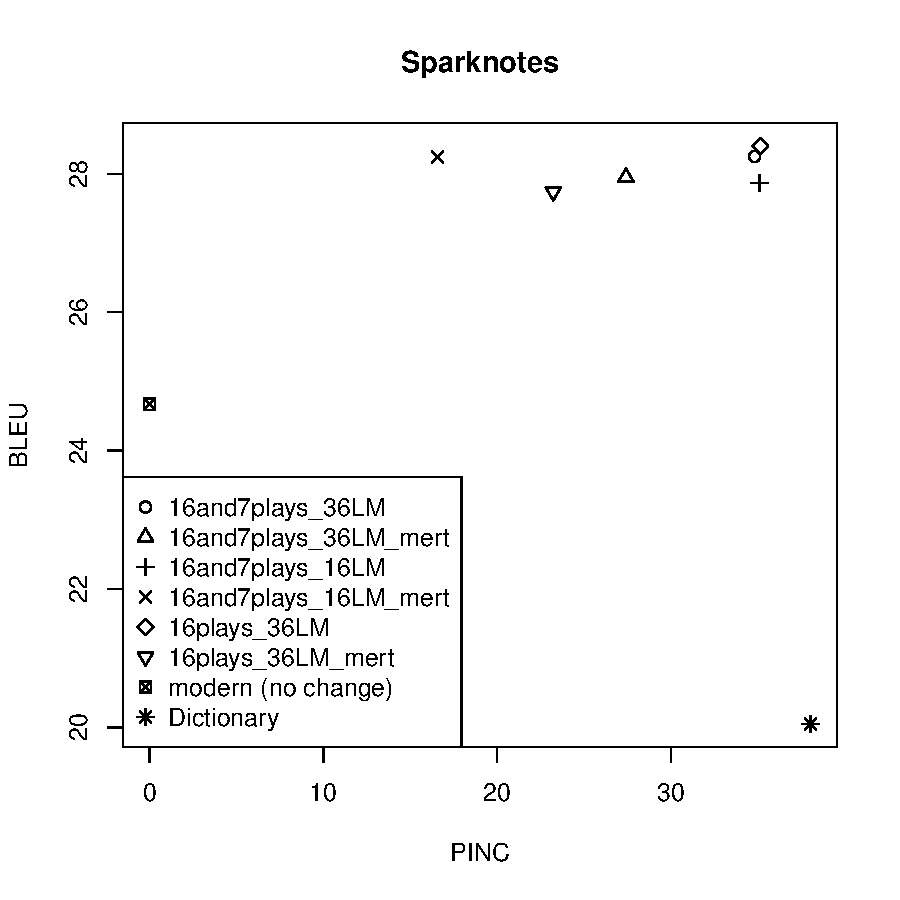
\includegraphics[width=2.4in]{figures/bleupinc1.pdf} & 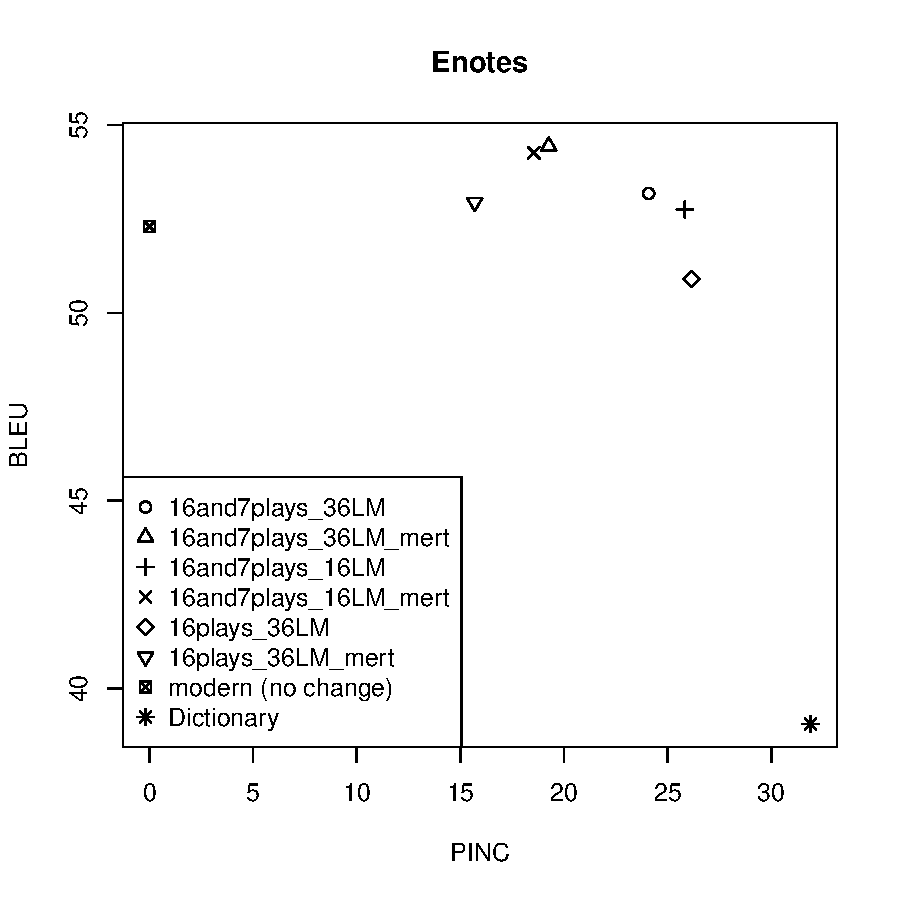
\includegraphics[width=2.4in]{figures/bleupinc2.pdf} \\
    \end{tabular}
  \end{center}
  \caption{Various Shakespearean paraphrase systems compared using BLEU and PINC.  A brief description of each system is presented in table \ref{systems}.}
  \label{bleupinc}
\end{figure}

\begin{table}[ht]
  \begin{center}
    \begin{tabular}{|l|l|p{1.4in}|p{1.4in}|}
      \hline
      Source & Speaker & Input & Output \\
      \hline
      \hline
      Romeo \& Juliet & Benvolio & He killed your relative, brave Mercutio, and then young Romeo killed him. & he slew thy kinsman , brave mercutio , and then young romeo kill him . \\
      \hline
      Romeo \& Juliet & Romeo & I can read my own fortune in my misery. & i can read mine own fortune in my woes . \\
      \hline
      Star Wars & Palpatine & If you will not be turned, you will be destroyed! & if you will not be turn 'd , you will be undone ! \\
      \hline
      Star Wars & Luke & Father, please! Help me! & father , i pray you , help me ! \\    
      \hline
      The Matrix & Agent Smith & Good bye, Mr. Anderson. & fare you well , good master anderson . \\
      \hline
      The Matrix & Morpheus & I'm trying to free your mind, Neo. But I can only show you the door. You're the one that has to walk through it. & i 'll to free your mind , neo. but i can but show you the door. you 're the one that hath to tread it . \\
      \hline
      Raiders of the Lost Ark & Belloq & Good afternoon, Dr. Jones. & well met , dr. jones . \\
      \hline
      Raiders of the Lost Ark & Jones & I ought to kill you right now. & i should kill thee straight . \\
      \hline
      %Terminator 2 & Terminator & My mission is to protect you. & my affair is to keep you . \\
      %\hline
      %Terminator 2 & Terminator & Negative. The T-1000's highest probability for success now would be to copy Sarah Connor and to wait for you to make contact with her. & negative. the t-1000 's most exalted probability for success now would be to have sarah connor and to stay for you to make contact with her . \\
      %\hline
      %Terminator 2 & Terminator & Skynet begins to learn at a geometric rate. ... In a panic, they try to pull the plug. & skynet begins to learn at a geometric rate. ... in a fearful sails , they would pluck the stop . \\
      %\hline
    \end{tabular}
  \end{center}
  \caption{Example Shakespearean paraphrases generated by the best overall system.}
  \label{examples}
\end{table}

\section{Human Evaluation}
\label{human_evaluation}
Figure \ref{bleupinc} provides some insight into the performance of the various systems, but it is initially unclear how well the BLEU and PINC
automatic evaluation metrics perform when applied to evaluating paraphrases that target a specific style of writing.  BLEU and PINC have previously
been shown to have high correlation with human judgments of semantic adequacy and lexical dissimilarity of paraphrase candidates, 
but the implications of this for the more specialized task of stylistic paraphrasing are unclear.

While BLEU is typically used to measure semantic adequacy, it seems reasonable to assume that it 
could also be useful for measuring stylistic alternations, since utterances
are more likely to contain overlapping ngrams if they are both semantically and stylistically similar.  What BLEU cannot tell us, however
is what portion of its improvements are due to stylistic similarity or semantic equivalence.  For this reason, we were motivated perform
an evaluation based on human judgments of semantic adequacy, lexical dissimilarity and stylistic similarity.

For this purpose, we randomly sampled 100 lines from {\em Romeo and Juliet}, then two of the authors annotated each sentence and its Shakespearean
translation to indicate semantic adequacy, lexical dissimilarity, stylistic similarity, and overall quality.
The aggregate results of the human evaluation are displayed in Figure \ref{human_judgements}.  Agreement between annotators
measured using Pearson's $\rho$ is displayed in Table \ref{annotator_agreement}.

Based on the human evaluation, it appears that the baseline combining paraphrases collected from Mechanical Turk \cite{chen11} with
a Shakespearean language model has the highest semantic adequacy, yet this approach is also fairly conservative in that it makes few changes to the input.

The dictionary baseline, and the paraphrase system trained on parallel modern translations are roughly comparable in terms of 
the number of changes made to the input, but the system trained on modern translations achieves higher semantic adequacy, while also being rated higher on style and overall.

These results are roughly in line with the automatic evaluation metrics presented in Figure \ref{bleupinc}.  However we also see several important
trends which are not apparent from the automatic evaluation.
Although the video baseline achieves the highest semantic adequacy in the human evaluation, its BLEU score
is significantly lower than 16plays\_36LM on the Sparknotes data.\footnote{
Note that the BLEU score of 16plays\_36LM is significantly lower when evaluated on the Enotes data.  This makes sense, because the 
16 plays come from Sparknotes. This system is not trained on the 7 Enotes plays which, whose modern translations tend
to be slightly different in style.}
It would appear that in this case BLEU is conflating semantic adequacy with writing style.  Although the paraphrases produced 
by the video baseline have high semantic adequacy, their style tends to differ substantially from the reference translations resulting
in fewer ngram matches, and thus a lower BLEU score.

\begin{table}
  \begin{center}
    \begin{tabular}{|l|l|l|l|}
      \hline
      Semantic Adequacy & Lexical Dissimilarity & Style & Overall \\
      \hline
      \hline
      0.73 & 0.82 & 0.64 & 0.62 \\
      \hline
    \end{tabular}
  \end{center}
  \caption{Agreement between annotators measured using Pearson's $\rho$.}
  \label{annotator_agreement}
\end{table}

\begin{figure}[ht]
  \begin{center}
    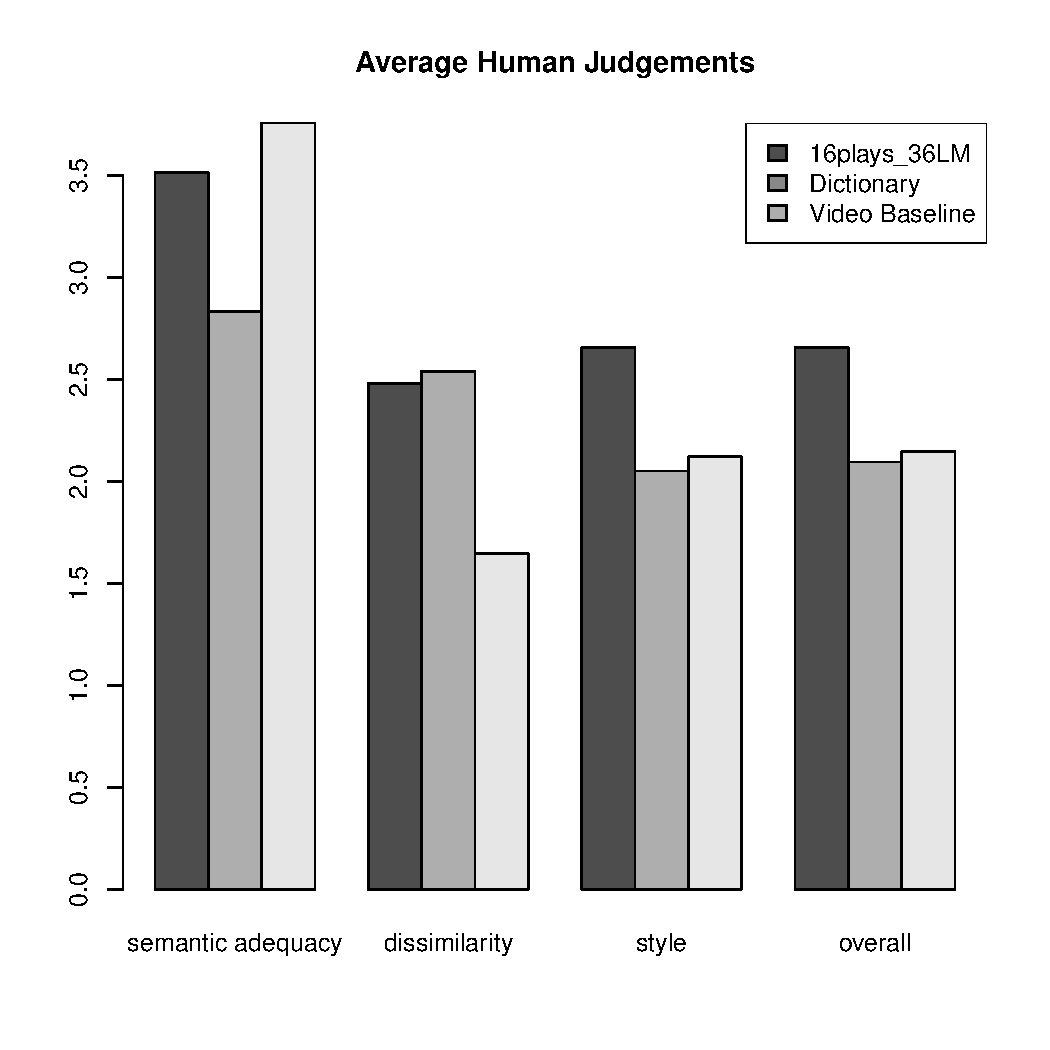
\includegraphics[width=5in]{figures/human_judgements.pdf}
  \end{center}
  \caption{Average human judgments evaluating semantic adequacy, lexical dissimilarity, stylistic similarity, and overall quality
    of Shakespearean paraphrase systems} 
  \label{human_judgements}
\end{figure}

\section{Automatic Metrics Evaluating Writing Style}
While PINC and BLEU do seem useful for automatically evaluating stylistic paraphrases, BLEU tends to conflate the notions of
semantic adequacy with writing style.  When comparing various systems using automatic metrics, it would seem useful
to separate the effects caused by these two distinct criteria.  We would like our automatic evaluation metrics to be able to distinguish
between a system which generates perfect paraphrases which do not match the target style of writing versus a system which
generates sentences in the correct style, but which convey different meaning.

To help address this issue we propose two new automatic evaluation metrics whose goal is to measure the degree to which
automatic paraphrases match the target style.  Both metrics assume existence of large corpora in both the source and
target style, but do not require access to any parallel text, or human judgments.

We present a preliminary evaluation of these metrics by measuring their correlation with human judgments, but
it should be emphasized that we are only evaluating these metrics with respect to one specific style of writing.  We
are optimistic that these results will generalize across writing styles, however, since they are based entirely
on ngram statistics.

\subsection{Cosine Similarity Style Metric}
As a first approach to automatic evaluation of writing style, we propose a vector-space model of similarity between the system
output and a large corpus of text in both the source and target style.  The intuition behind this metric is that  a large ngram
overlap between the system's output and a corpus of text in the target style should indicate that the
output is likely to be stylistically appropriate.

More concretely, we extract ngrams from both the source and target corpus which are represented as binary
vectors $\vec{s}$, and $\vec{t}$; similarly the output sentence is represented using a vector of
ngrams $\vec{o}$.  
The proposed metric is the normalized cosine similarity between the source and target corpora:
\[
S_{\text{Cosine}}(\vec{o}) = \frac{\frac{\vec{o} \cdot \vec{t}}{\|\vec{o}\| \times \|\vec{t}\|}}{\frac{\vec{o} \cdot \vec{t}}{\|\vec{o}\| \times \|\vec{t}\|} + \frac{\vec{o} \cdot \vec{s}}{\|\vec{o}\| \times \|\vec{s}\|}}
\]
 

\subsection{Logistic Regression Style Metric}
We also consider an approach to measuring style which is based on logistic regression as opposed to cosine similarity.
%We also consider a logistic Regression based approach as an alternative to cosine similarity.
Here the idea is to estimate the probability that each
sentence belongs to the target style based on the ngrams it contains, using large corpora of \emph{in domain} and \emph{out-of domain} sentences to learn  parameters of a logistic regression model.

The probability that a sentence belongs to the target style is estimated as follows:
\[
%P(\text{style} = \text{target}|\text{output}) \propto \text{exp} \left( \vec{\theta} \cdot \vec{f(\text{output})} \right)
P(\text{style} = \text{target}|\text{sentence}) = \frac{1}{1 + e^{-\left( \vec{\theta} \cdot \vec{f(\text{sentence})} \right)}}
\]
Where $\vec{f(\text{sentence})}$ is a vector of ngrams contained by the sentence, and $\vec{\theta}$ is a vector of weights corresponding to each possible ngram.

The parameters, $\vec{\theta}$, are optimized to maximize conditional likelihood on the source and target corpus, where the assumption is that the target corpus
is in the target style, whereas the source corpus is not.\footnote{
  Parameters were optimized using MEGAM \url{http://www.cs.utah.edu/~hal/megam/}.
}

\subsection{Evaluation}
We trained both the logistic regression and cosine similarity evaluation metrics using the original Shakespeare plays and modern translations as
the source and target corpus respectively, then measured Pearson's Correlation Coefficient between the automatic
evaluation metrics and human judgments described in \S \ref{human_evaluation}.  These results are reported in table \ref{correlation}.

\begin{table}
  \begin{center}
  \begin{tabular}{|l|l|r|}
    \hline
    & & Pearson's $\rho$ \\
    \hline
    \hline
    semantic adequacy & BLEU & 0.35 \\
    \hline
    dissimilarity & PINC & 0.78 \\
    \hline
    style & BLEU & 0.07 \\
    \hline
    style & PINC & 0.20 \\
    \hline
    style & Cosine & 0.37 \\
    \hline
    style & Logistic regression & 0.47 \\
    \hline
  \end{tabular}
  \end{center}
  \caption{Correlation between various human judgments and automatic evaluation metrics}
  \label{correlation}
\end{table}

As can be seen in table \ref{correlation}, the correlation between semantic adequacy and BLEU appears smaller than that reported in previous work \cite{chen11}.  Presumably this is
due to the conflation of stylistic differences and semantic adequacy discussed in \S \ref{human_evaluation}.  However it also appears 
that the correlation between BLEU and human style judgments is too low to be of practical use for evaluating style.

PINC, on the other hand has high correlation with judgments on dissimilarity, and is also moderately correlated with human style
judgments.  We believe PINC has some correlation with writing style, because the systems we are evaluating all target Shakespearean English, 
so whenever changes are made to the input, they are likely to make it similar to the target style.
Although PINC has relatively high correlation with human judgments, it is likely not a very useful measure of writing style in practice.
For example, consider a paraphrase system which makes many changes to the input and thus gets a high PINC score, but targets a completely different writing style.

Both the cosine and logistic regression style metrics achieve the highest overall correlation with human writing style judgments, with the logistic regression style score performing best.

We note that overall the automatic metrics tend to agree with agree with human judgments as displayed in Figure \ref{style_metrics}.\footnote{
  Although the automatic style metrics rate the dictionary system higher than the video corpus baseline, both systems have very comparable
  style scores in the automatic and human evaluations.
}

\begin{figure}
  \begin{center}
    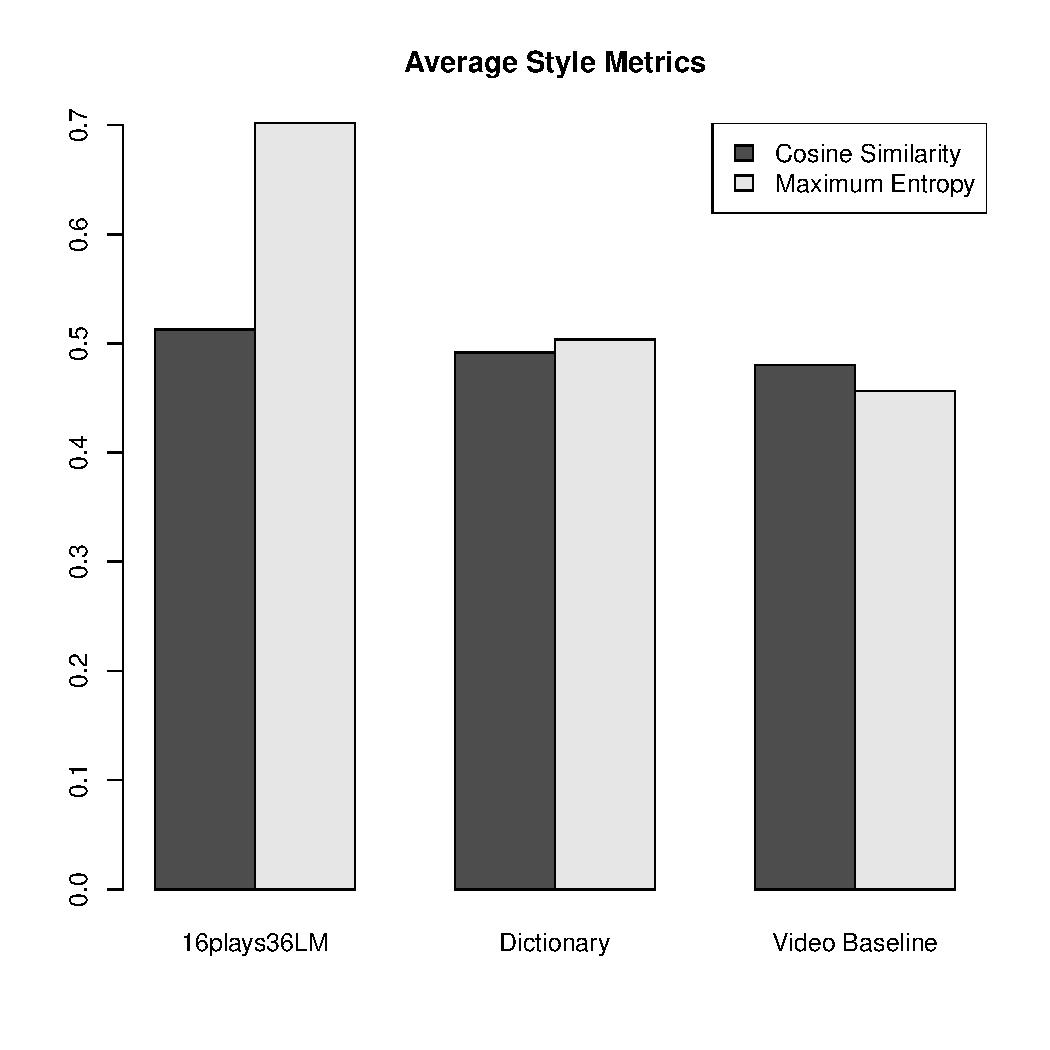
\includegraphics[width=5in]{figures/style_metrics.pdf}
    \end{center}
    \caption{Results comparing the 3 systems using the automatic style metrics.}
    \label{style_metrics}
\end{figure}

\section{Translating Shakespeare's Plays to Modern English}
Finally we perform a preliminary evaluation on the task of automatically translating Shakespeare's plays into modern English.  
%Success at this task could have immediate benefits to students, as well as translators of Shakespeare's plays into modern English. 

For the purposes of this evaluation, 
we make use of the same paraphrase systems previously described, but swap the source and target languages.
Additionally, each system makes use of a language model constructed from the 16 modern translations, with {\em Romeo and Juliet} held out for testing.  
510 lines from {\em Romeo and Juliet} were automatically translated into modern English using each system, and the aligned modern 
translations were used as a reference when computing BLEU.  The results of evaluating each of the automatic evaluation metrics on this
data are presented in Figure \ref{shakespeare_to_modern_automatic}.  

These results suggest that in comparison to the dictionary and video corpus baselines, 
our system trained on modern translations generates a large number of paraphrases which match the target style.
Note that the paraphrase system 
based on the out-of-domain video corpus makes very few changes to the input, and thus achieves a very low PINC score.  This is due to the many out of
vocabulary words in Shakespeare's plays which result in very few matching source phrases in the video baseline's phrase table.

While we have yet to perform a human evaluation on the task of paraphrasing Shakespeare's plays into modern English, 
informal inspection of the resulting translations is encouraging.  Several automatic paraphrases into modern English are presented in Table \ref{modern_examples}.

\begin{figure}
  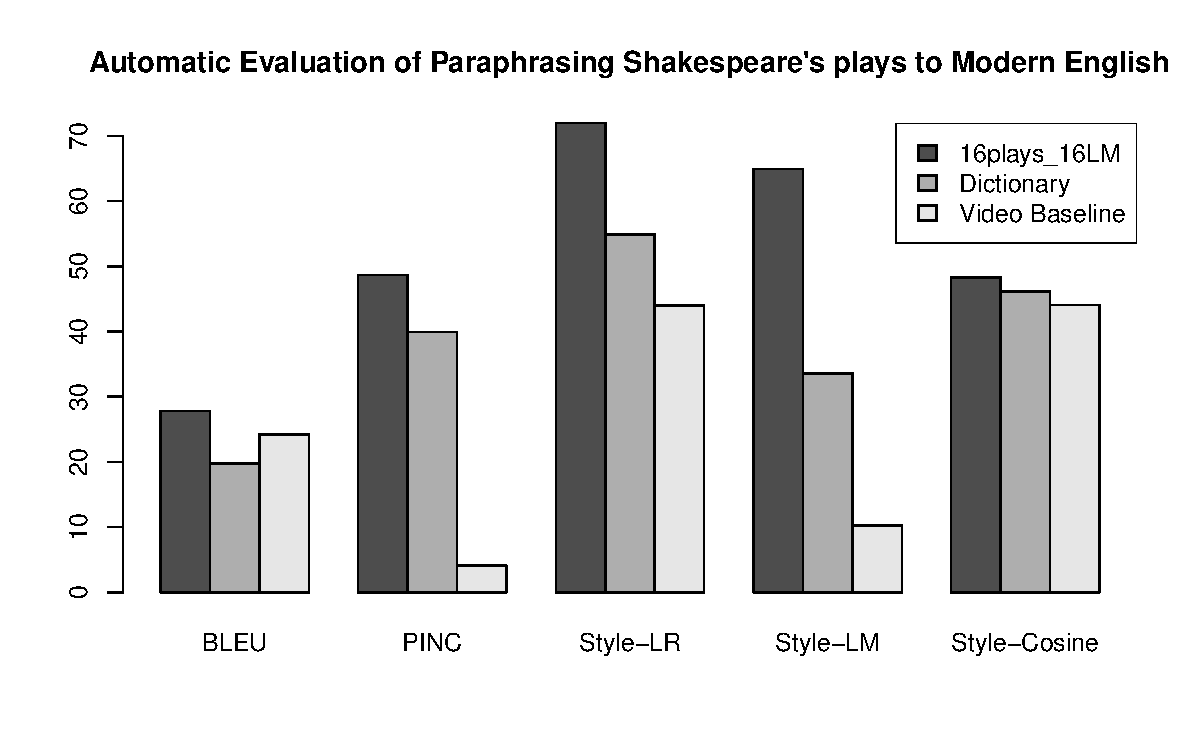
\includegraphics[width=5in]{figures/shakespeare_to_modern.pdf}
  \caption{Automatic evaluation of paraphrasing Shakespeare's plays into modern English comparing a system based on parallel text (16plays\_16LM), 
  a Dictionary baseline, and a system trained on out of domain parallel monolingual text.  Note that the video corpus baseline achieves low overall
  PINC score, as few phrases in the input match phrases found in its phrase table, resulting in a small number of changes to the input.}
  \label{shakespeare_to_modern_automatic}
\end{figure}

\begin{table}
  \begin{center}
  \begin{tabular}{|l|p{1.8in}|p{1.8in}|}
    \hline
    Speaker & Input & Output \\
    \hline
    \hline
    MERCUTIO & i will bite thee by the ear for that jest . & i ’ ll bite you by the ear for that joke . \\
    \hline
    MONTAGUE & what further woe conspires against mine age ? & what ’ s true despair conspires against my old age ? \\
    \hline
    ROMEO & how doth my lady ? & how is my lady ? \\
    \hline
    FRIAR LAURENCE & hast thou slain tybalt ? & have you killed tybalt ? \\
    \hline
    NURSE & an i might live to see thee married once , i have my wish . & if i could live to see you married , i ’ ve my wish . \\
    \hline
    PRINCE & benvolio , who began this bloody fray ? & benvolio , who started this bloody fight itself ? \\
    \hline
    JULIET & what is your will ? & what do you want ? \\
    \hline
    LADY CAPULET & call her forth to me . & bring her out to me . \\
    \hline
  \end{tabular}
  \end{center}
  \caption{Example modern paraphrases of lines from Romeo and Juliet generated using our system.}
  \label{modern_examples}
\end{table}

\section{Related Work}
Much previous work has addressed the task of automatically generating paraphrases \cite{Barzilay03,dolan04,Shinyama03,Das09,bannard05,Callison-Burch08,Kok10}.  
In addition several authors have previously proposed 
automatic metrics specifically for evaluating paraphrases \cite{chen11,Callison-Burch08b,liu10}.
We are not aware, however, of any work that has addressed the task of generating or evaluating
paraphrases targeting a specific style of writing.

Perhaps most relevant, however, is recent work automatic generation of rhythmic poetry \cite{Greene10}.  This work focuses on automatically generating and translating
poetry in an appropriate meter (e.g. iambic pentameter) using finite-state transducers, but does not investigate the task of paraphrase.  Their generation system
is trained on Shakespeare's sonnets, and they investigate the task of automatically translating Dante's Divine Comedy from Italian to English.
While our work does not address the issue of meter, it should be possible to combine our translation
models with their weighted finite state transducers to produce Shakespearean paraphrase models which produce output in an appropriate meter.

Finally we highlight related work on authorship classification which can be seen as detecting a specific style of writing \cite{Gamon04,Raghavan10}.
This work has not specifically addressed the task of automatically generating or evaluating paraphrases in a specific style, however.

\section{Conclusions}
We have presented the first investigation into the task of automatic paraphrasing while targeting a specific writing style.  Using Shakespeare's plays and their
modern translations as a tesbed for this task, we developed a series of paraphrase systems targeting Shakespearean English.  We showed that while existing evaluation
metrics are useful for evaluating paraphrases in this context, BLEU tends to conflate semantic equivalence with writing style and thus gives an incomplete picture of 
system performance on these different dimensions.

To address this problem, we introduced two new metrics for evaluating writing style, one based on cosine similarity and the other based on logistic regression.
We measured correlation between automatic metrics and human judgments, and showed
that our new metrics have better correlation with human judgments than existing metrics in the context of our task.
While this evaluation is limited to one specific style of writing, we are optimistic that these or similar metrics will also perform well when
evaluating paraphrase systems targeting other writing styles.

Finally, we applied these automatic evaluation metrics in an initial investigation into the task of translating Shakespeare's plays into modern English.
%We plan to translate the remaining 20 of Shakespeare's plays, which could be beneficial to students
%of Shakespeare and also to human translators.

\bibliographystyle{apa}
\bibliography{paper}

%%================================================================
\end{document}
